\documentclass[11pt,a4paper]{article}
\usepackage[T1]{fontenc}
\usepackage[utf8]{inputenc}
\usepackage{tgpagella}
\usepackage{amsmath,amsthm}
\usepackage{newpxmath}
\usepackage[scale=.94]{tgheros}
\usepackage{inconsolata}
\usepackage[a4paper,margin=25mm,headheight=15pt]{geometry}
\usepackage{amsmath,amsthm,mathtools,booktabs,array,longtable}
\usepackage{microtype,graphicx,xcolor,titlesec,fancyhdr}
\usepackage[most]{tcolorbox}
\usepackage{enumitem,listings}
\usepackage[colorlinks=true,linkcolor=Forest,citecolor=Forest,urlcolor=Forest]{hyperref}
\usepackage{aliascnt}
\usepackage[nameinlink,noabbrev]{cleveref}
\definecolor{Forest}{HTML}{294D3D}
\definecolor{OliveLight}{HTML}{F0F2E7}
\definecolor{InkGray}{HTML}{555D57}
\titleformat{\section}{\Large\sffamily\bfseries\color{Forest}}{\thesection}{.7em}{}
\titleformat{\subsection}{\large\sffamily\bfseries\color{Forest}}{\thesubsection}{.65em}{}
\titlespacing*{\section}{0pt}{2.1ex plus 1ex minus .2ex}{1ex plus .2ex}
\titlespacing*{\subsection}{0pt}{1.7ex plus .6ex minus .2ex}{.7ex plus .2ex}
\pagestyle{fancy}\fancyhf{}
\fancyhead[L]{\small\sffamily\color{InkGray}Strict growth of adjacency-bounded avoiders}
\fancyhead[R]{\small\sffamily\color{InkGray}Research report}
\fancyfoot[C]{\small\sffamily\thepage}
\renewcommand{\headrulewidth}{.25pt}
\newtheorem{theorem}{Theorem}[section]
\newaliascnt{lemma}{theorem}
\newtheorem{lemma}[lemma]{Lemma}
\aliascntresetthe{lemma}
\newaliascnt{proposition}{theorem}
\newtheorem{proposition}[proposition]{Proposition}
\aliascntresetthe{proposition}
\newaliascnt{corollary}{theorem}
\newtheorem{corollary}[corollary]{Corollary}
\aliascntresetthe{corollary}
\theoremstyle{definition}\newaliascnt{definition}{theorem}
\newtheorem{definition}[definition]{Definition}
\aliascntresetthe{definition}
\theoremstyle{remark}\newaliascnt{remark}{theorem}
\newtheorem{remark}[remark]{Remark}
\aliascntresetthe{remark}
\newtcolorbox{resultbox}{enhanced,breakable,colback=OliveLight,colframe=Forest,
  boxrule=.45pt,arc=1mm,left=3mm,right=3mm,top=2mm,bottom=2mm}
\newcommand{\Av}{\operatorname{Av}}
\newcommand{\spr}{\operatorname{spr}}
\newcommand{\Cat}{\mathcal C}
\newcommand{\Aclass}{\mathcal A}
\newcommand{\preceqc}{\preceq}
\newcommand{\eps}{\varepsilon}
\newcommand{\one}{\mathbf 1}
\newcommand{\N}{\mathbb N}
\newcommand{\R}{\mathbb R}
\newcommand{\shift}{\Phi}
\newcommand{\dd}{\mathrm d}
\allowdisplaybreaks[2]
\setlength{\parindent}{1.1em}
\setlength{\parskip}{.25em}
\setlist{nosep,leftmargin=1.5em}
\lstset{basicstyle=\small\ttfamily,breaklines=true,columns=fullflexible,
  keepspaces=true,frame=single,rulecolor=\color{InkGray},xleftmargin=1mm,xrightmargin=1mm}
\hypersetup{pdftitle={Strict growth and the Catalan limit for adjacency-bounded 132-avoiding permutations},
 pdfauthor={AI-assisted research report prepared for Vladimir Reshetnikov},
 pdfsubject={A proof of strict monotonicity and a two-term asymptotic expansion}}

\begin{document}
\thispagestyle{empty}
\begin{center}
{\small\sffamily\color{Forest}\bfseries COMBINATORICS\quad /\quad INTEGER SEQUENCES\quad /\quad ASYMPTOTICS}\par
\vspace{8mm}
{\LARGE\bfseries Strict growth and the Catalan limit\par
for adjacency-bounded\par
132-avoiding permutations}\par
\vspace{5mm}
{\large A proof of the remaining strict-growth conjecture\par
and a two-term large-bound asymptotic}\par
\vspace{5mm}
{\sffamily Research report prepared for Vladimir Reshetnikov}\par
{\small September 19, 2026}
\end{center}
\vspace{3mm}
\begin{abstract}
Let $a_n^{(m)}$ count permutations $\pi\in S_n$ avoiding the pattern $132$ and
satisfying $|\pi_{i+1}-\pi_i|\le m$. Nadler conjectured that their exponential
growth constants increase strictly from $1$ to $4$. Mayama and Akita established
a finite-state enumeration, the existence of the growth constants,
non-strict monotonicity, and convergence to $4$. We prove the missing strict
inequality for every adjacency bound. The argument embeds each of the two
irreducible cyclic state components at bound $m$ into a proper principal
submatrix of its counterpart at bound $m+1$ by increasing both finite endpoint
thresholds by one. Perron--Frobenius comparison then gives strict growth in
\emph{each} component, independently of which component dominates.

A separate counting argument gives
\[
 4-\alpha_m=\frac{2\log m+4\log\log m+O(1)}{m}.
\]
It compares the full class with a scalar Catalan majorant and an injectively
encoded family of variable-length skew blocks. A truncated-series root lemma
also bounds the possible constant term. Complete proofs, exact generating
functions for $m\le4$, integer sequences, and independently checked rational
Perron certificates accompany the report.
\end{abstract}
\begin{resultbox}
\textbf{Scope and attribution.}
The finite-state system and fixed-$m$ spectral description are established
work, not claimed as new here. The contributions developed in this report
are the all-$m$ strict comparison and the refined asymptotic bounds. A targeted
literature check found no later resolution of the strict inequality in the
sources inspected. This is a research proof with reproducible checks, not a
claim of external peer review or an exhaustive novelty certification.
\end{resultbox}
\vfill
{\small\sffamily\color{InkGray}Companion archive: editable \texttt{article.tex}, compiled PDF,
standard-library exact verifier, numerical and symbolic computation scripts,
certificate files, and CSV tables.}
\newpage
\tableofcontents
\newpage

\section{The problem and the results}
\label{sec:results}
A permutation $\pi\in S_n$ avoids $132$ when there are no indices $i<j<k$ for
which $\pi_i<\pi_k<\pi_j$. Fix an integer $m\ge1$ and put
\[
\Aclass_n^{(m)}=\{\pi\in\Av_n(132):|\pi_{i+1}-\pi_i|\le m
                  \text{ for }1\le i<n\},\qquad
 a_n^{(m)}=|\Aclass_n^{(m)}|.
\]
We set $a_0^{(m)}=1$ and use the ordinary generating function
\[
 A_m(x)=\sum_{n\ge0}a_n^{(m)}x^n.
\]
The growth constant is
\begin{equation}
 \alpha_m=\lim_{n\to\infty}(a_n^{(m)})^{1/n}.
 \label{eq:alpha}
\end{equation}
The order of limits matters: $n\to\infty$ is taken for each fixed $m$, and
only afterwards do we let $m\to\infty$. The trivial identity
$a_n^{(m)}=C_n$ for $m\ge n-1$ does not by itself settle this iterated limit.
Here $C_n=\binom{2n}{n}/(n+1)$ is the $n$th Catalan number.

\subsection{Which part was still open?}
Nadler's Conjecture~2 in Section~5.2 of \cite{Nadler} asks for the existence of
\eqref{eq:alpha}, strict increase $1=\alpha_1<\alpha_2<\cdots<4$, and limit $4$.
Mayama and Akita subsequently proved rationality for all $m$, existence of the
limit, non-strict increase, and $4-\alpha_m=O(\log m/m)$
\cite[Theorems~2.4, 4.12, and 4.14]{MayamaAkita}. Their monotonicity theorem
states $\alpha_m\le\alpha_{m+1}$, not strict inequality.

Merely finding additional permutations at bound $m+1$ is insufficient:
sequences $2^n$ and $2^n+1$ differ strictly at every index but have identical
exponential growth. The needed argument must show that the extra freedom
changes the exponential rate.

\begin{theorem}[Strict increase]\label{thm:strict-main}
For every integer $m\ge1$,
\[
 \alpha_{m+1}>\alpha_m.
\]
In the two-component spectral representation described below, both component
rates increase strictly: for every $m\ge2$,
\[
 \lambda_U(m+1)>\lambda_U(m),\qquad
 \lambda_V(m+1)>\lambda_V(m).
\]
Consequently Nadler's growth-constant conjecture holds in full.
\end{theorem}

\begin{theorem}[Two-term approach to the Catalan limit]\label{thm:asympt-main}
As $m\to\infty$ through integers,
\begin{equation}
 4-\alpha_m=\frac{2\log m+4\log\log m+O(1)}{m}.
 \label{eq:main-asympt}
\end{equation}
In particular, $4-\alpha_m\sim2\log m/m$. All logarithms in this report are
natural logarithms.
\end{theorem}

\begin{theorem}[A window for the next constant]\label{thm:window-main}
Define $E_m=m(4-\alpha_m)-2\log m-4\log\log m$ for $m\ge2$. Then
\begin{equation}
 2\log\pi-4\log2
 \ \le\ \liminf_{m\to\infty}E_m
 \ \le\ \limsup_{m\to\infty}E_m
 \ \le\ 2\log\pi.
 \label{eq:constant-window}
\end{equation}
No convergence of $E_m$ is asserted.
\end{theorem}

The strict comparison uses a finite-state embedding. The asymptotic results
use scalar comparison series and do not require deciding which finite-state
component has the larger rate. The distinction is important: the all-$m$
comparison of $\lambda_U(m)$ with $\lambda_V(m)$ is a separate question.

\section{The exact endpoint recursion}
\label{sec:endpoints}
This section develops the endpoint representation of Mayama and Akita
\cite[Section~2]{MayamaAkita}, including the counting details needed later.
It is included to make the subsequent proofs independently readable.

\subsection{Decomposition at the maximum}
If $\pi=L\,n\,R$ avoids $132$, every entry of $L$ exceeds every entry of $R$:
otherwise an entry of $L$, then $n$, then an entry of $R$ forms $132$.
Conversely, if this separation holds and both standardized sides avoid
$132$, their concatenation with $n$ avoids $132$.

Suppose $R$ is nonempty and the maximum is at position $k$. Then $L$ has
length $k-1$, its values are $n-k+1,\ldots,n-1$, and $R$ has values
$1,\ldots,n-k$. The jump from $n$ to the first entry of $R$ is at least $k$.
Therefore
\begin{equation}
 R\ne\varnothing\quad\Longrightarrow\quad 1\le k\le m.
 \label{eq:max-position}
\end{equation}
The alternative $R=\varnothing$ means appending the maximum to an avoider
of length $n-1$.

\subsection{Cumulative endpoint thresholds}
Let
\[
 B_m=\{0,1,\ldots,m-1,\infty\}.
\]
For $p,q\in B_m$, let $T_{p,q}^{(m)}(n)$ count the permutations in
$\Aclass_n^{(m)}$ satisfying
\[
 n-\pi_1\le p,\qquad n-\pi_n\le q.
\]
A threshold $\infty$ imposes no restriction. Define
\[
 F_{p,q}^{(m)}(x)=\sum_{n\ge1}T_{p,q}^{(m)}(n)x^n.
\]
A negative threshold gives the zero series, and $\infty-k=\infty$.
We suppress the superscript $(m)$ where it is fixed.

For $k\ge2$ define the nonnegative integer
\begin{equation}
 c_{k,p}=\bigl|\{\sigma\in\Av_{k-1}(132):k-\sigma_1\le p\}\bigr|,
 \qquad c_{1,p}=1
 \label{eq:c-def}
\end{equation}
for nonnegative or infinite $p$; for negative $p$ set $c_{k,p}=0$.
These coefficients do not otherwise depend on $m$. Two properties will be
crucial:
\begin{equation}
 c_{k,p+1}\ge c_{k,p},\qquad c_{k,\infty}=C_{k-1}.
 \label{eq:c-monotone}
\end{equation}
For finite $p\ge0$ and $k\ge2$, an explicit formula is
\begin{equation}
 c_{k,p}=\sum_{j=1}^{\min(p,k-1)}
 \frac{j}{k-1}\binom{2k-j-3}{k-2}.
 \label{eq:c-formula}
\end{equation}
A generating-function proof of this formula appears in
\cref{sec:block-weights}; no numerical fitting is involved.

\begin{proposition}[Endpoint recurrence]\label{prop:endpoint}
For all $p,q\in B_m$,
\begin{equation}
 F_{p,q}=x+\sum_{k=1}^m c_{k,p}x^kF_{m-k,q-k}
                   +xF_{p-1,m-1}.
 \label{eq:endpoint}
\end{equation}
Moreover $A_m(x)=1+F_{\infty,\infty}(x)$.
\end{proposition}
\begin{proof}
The singleton permutation contributes $x$ to every nonnegative threshold
state. For length at least two, first suppose $R\ne\varnothing$ in the
maximum decomposition. By \eqref{eq:max-position}, $k\le m$.
The left block has $k-1$ values in an interval of that length, so its internal
jumps, and its jump to $n$, are automatically at most $m$. Its first-entry
restriction gives $c_{k,p}$ choices; for $k=1$ the first entry is $n$ and the
left block is empty.

The right block has length $n-k$. Writing its first and last entries as
$R_1$ and $R_{n-k}$, the two remaining restrictions are exactly
\[
 (n-k)-R_1\le m-k,\qquad
 (n-k)-R_{n-k}\le q-k.
\]
The first inequality is the jump bound from $n$ to $R_1$; the second is the
last-entry threshold for the whole permutation. This gives
$c_{k,p}x^kF_{m-k,q-k}$.

If $R=\varnothing$, remove the final maximum. The first deficiency increases
by one when the maximum is appended, giving threshold $p-1$ for the smaller
permutation. Its last deficiency must be at most $m-1$ to permit the last
jump. The final entry of the whole permutation is $n$, so any nonnegative
$q$ is satisfied. This is $xF_{p-1,m-1}$. The cases are disjoint and reversible.
\end{proof}

Let $W_m(x)$ have rows and columns indexed by $B_m^2$, with
\begin{align}
 (W_m)_{(p,q),(r,s)}={}&
  \sum_{k=1}^m c_{k,p}x^k
       \mathbf1_{(r,s)=(m-k,q-k)}\notag\\
 &+x\,\mathbf1_{(r,s)=(p-1,m-1)}.
 \label{eq:matrix}
\end{align}
Invalid negative thresholds are omitted. Rows are the left-hand states of
\eqref{eq:endpoint}; columns are the right-hand states. Thus
\begin{equation}
 F=x\one+W_m(x)F,
 \qquad F=x(I-W_m(x))^{-1}\one.
 \label{eq:matrix-system}
\end{equation}
Every entry of $W_m$ has zero constant term, so the inverse is well-defined
as a formal power series. This also proves rationality and gives an exact
algorithm for computing $A_m$.

\section{Cyclic components and growth constants}
\label{sec:components}
The following fixed-$m$ structure is established in
\cite[Proposition~2.7 and Theorem~4.12]{MayamaAkita}. We supply elementary
component and transfer-graph arguments to make the spectral input explicit.

\subsection{The two relevant components}
For $m\ge2$ put
\begin{align}
 U_m&=\{(p,\infty):0\le p\le m-1\},\label{eq:U}\\
 V_m&=\{(p,q):0\le q<p\le m-1\}
       \ \cup\ \{(p,m-1):0\le p\le m-2\}.
       \label{eq:V}
\end{align}
Their sizes are $m$ and $(m-1)(m+2)/2$. Write $W_{U_m}$ and $W_{V_m}$ for the
corresponding principal matrices. A directed edge means a nonzero term in a
row of \eqref{eq:matrix}, directed from its row state to its column state.

\begin{lemma}[Component structure]\label{lem:components}
At every real $x>0$, both $W_{U_m}(x)$ and $W_{V_m}(x)$ are irreducible.
The only other cyclic component of the full state graph is the singleton
$I_m=(\infty,m-1)$, whose internal matrix is $(x)$. Each of these three
components is reachable from $(\infty,\infty)$.
\end{lemma}
\begin{proof}
Within $U_m$, every state has a $k=1$ edge to $(m-1,\infty)$. From that state,
the $k=1,\ldots,m$ edges reach every state of $U_m$, since
$c_{k,m-1}>0$. Hence $U_m$ is strongly connected.

For $V_m$, call the states with $q<p$ lower states and the states
$(p,m-1)$ top states. Every lower state has an append edge to a top state.
Every top state has a $k=1$ edge to
\[
 e=(m-1,m-2).
\]
It remains to show that $e$ reaches every state. For $m=2$ this is the
immediate two-state cycle. Suppose $m\ge3$. Appending at $e$ reaches
$(m-2,m-1)$; its split edges reach all lower states $(p,p-1)$, $1\le p\le m-1$.
Their append edges reach every top state. Inductively, suppose all lower
states of gap at most $d-1$ are reachable, where $2\le d\le m-1$.
The state $(m-1,m-d)$ is then reachable. Its split edge with $k=m-p$ reaches
$(p,p-d)$ for every $d\le p\le m-1$. Thus every lower gap is reached.

For finite $q$, every valid split edge ends at a lower state, because
$(m-k)-(q-k)=m-q>0$. Every valid append edge with finite $p$ ends at a top
state. Therefore a finite--finite state outside $V_m$ cannot be on a cycle.
A state $(\infty,q)$ with finite $q$ has append target $I_m$ and split
targets in $V_m$; among these states only $I_m$ has a self-loop. No edge
returns to $(\infty,\infty)$. Edges with second coordinate $\infty$ stay
in $U_m$ or leave it by an append edge, and cannot return from a finite
second coordinate. This exhausts all possibilities.

Finally, the $k=1$ split from $(\infty,\infty)$ reaches $U_m$, its append
edge reaches $I_m$, and a $k=1$ split from $I_m$ reaches $e\in V_m$.
\end{proof}

\subsection{The strict matrix comparison used in the proof}
We use the Perron--Frobenius theorem for finite nonnegative matrices: an
irreducible matrix has positive left and right eigenvectors at its spectral
radius; a primitive matrix has powers asymptotic to a positive rank-one
matrix times the corresponding power of that radius.

\begin{lemma}[Proper principal comparison]\label{lem:PF}
Let $M$ be an irreducible nonnegative matrix and let $S$ be a nonempty proper
subset of its indices. If $B=M[S,S]$, then $\spr(B)<\spr(M)$.
If $0\le N\le B$ entrywise, then $\spr(N)<\spr(M)$ as well.
\end{lemma}
\begin{proof}
Take a nonnegative nonzero Perron vector $v$ of $B$ and extend it by zeros to
a vector $w$ on all indices of $M$. Then $Mw\ge\spr(B)w$. There is strict
inequality in at least one coordinate: the support of $w$ is nonempty and
proper, and irreducibility supplies an edge from its complement to that
support. If $u$ is a positive left Perron vector of $M$, multiplication by
$u^{\mathsf T}$ gives
\[
 \spr(M)u^{\mathsf T}w>\spr(B)u^{\mathsf T}w.
\]
Since $u^{\mathsf T}w>0$, the first assertion follows. Entrywise monotonicity
of the spectral radius gives $\spr(N)\le\spr(B)$; for example, this
monotonicity follows by comparing powers and then taking matrix-norm roots.
\end{proof}

For $C=U,V$, there is a unique $r_C(m)>0$ satisfying
\begin{equation}
 \spr(W_{C_m}(r_C(m)))=1,
 \qquad \lambda_C(m)=r_C(m)^{-1}.
 \label{eq:component-root}
\end{equation}
Indeed the spectral radius is continuous, tends to zero as $x\downarrow0$,
and tends to infinity as $x\to\infty$ because the component has a positive
cycle. If $y>x>0$, every monomial has degree at least one, so
$W_{C_m}(y)\ge(y/x)W_{C_m}(x)$. Its positive spectral radius is therefore
strictly increasing.

\begin{proposition}[Fixed-bound growth]\label{prop:growth}
For $m\ge2$ the limit \eqref{eq:alpha} exists and
\begin{equation}
 \alpha_m=\max\{\lambda_U(m),\lambda_V(m)\}.
 \label{eq:alpha-max}
\end{equation}
Also $\lambda_U(m)>1$.
\end{proposition}
\begin{proof}
The state $(m-1,\infty)$ has an internal self-loop of weight $x$.
At $x=1$ its singleton principal matrix is $(1)$, and it is a proper
principal matrix of $W_{U_m}(1)$. By \cref{lem:PF}, the latter has spectral
radius greater than one. Thus $r_U(m)<1$ and $\lambda_U(m)>1$.

To justify the actual limit rather than only a limsup, replace each edge
of weight $c x^k$ by a directed path of $k$ unit-length edges with total
multiplicity $c$. Use fresh intermediate vertices for every edge. Let $H$
be the resulting finite nonnegative adjacency matrix, and let $b$ be one
on original endpoint states and zero on intermediate states. With $o$ the
state $(\infty,\infty)$, \eqref{eq:matrix-system} gives
\[
 a_n^{(m)}=e_o^{\mathsf T}H^{n-1}b\qquad(n\ge1).
\]
For an expanded irreducible component with Perron eigenvalue $\lambda$,
eliminating the intermediate coordinates of a positive eigenvector gives
$z=W_{C_m}(1/\lambda)z$. Its eigenvalue is therefore $\lambda_C(m)$.
The expanded singleton component has eigenvalue one. The component
classification and $\lambda_U(m)>1$ show that $\spr(H)$ is the right-hand
side of \eqref{eq:alpha-max}.

The expanded $U_m$ component is primitive, since it is strongly connected
and has a length-one loop. For $m\ge3$, the expanded $V_m$ component has
closed walks of lengths two and five. The first is
\[
 e\ \xrightarrow{1}\ (m-2,m-1)\ \xrightarrow{1}\ e.
\]
For the second, split with $k=2$ on the middle state and then append and
split with $k=1$:
\[
 e\xrightarrow{1}(m-2,m-1)
 \xrightarrow{2}(m-2,m-3)
 \xrightarrow{1}(m-3,m-1)
 \xrightarrow{1}e.
\]
The labels are edge lengths. All coefficients are positive, including
when $m=3$. Their greatest common divisor is one, so this component is
primitive. When $m=2$, $V_m$ is a two-cycle with rate one and is not dominant.

A dominant primitive component is reachable from $o$, and $b$ is positive
on its original states. Fixing an entrance path and then applying the
primitive Perron theorem supplies $a_n^{(m)}\ge c\spr(H)^n$ for all
sufficiently large $n$, with $c>0$. A finite-matrix power bound gives
$a_n^{(m)}\le C n^D\spr(H)^n$ for some fixed $C,D$ (or, equivalently, an
upper bound by $(\spr(H)+\eps)^n$ for each $\eps>0$).
Taking $n$th roots proves \eqref{eq:alpha-max} and the existence of the limit.
\end{proof}

\section{A shift of endpoint thresholds proves strict increase}
\label{sec:strict}
The key comparison preserves the split length $k$, not merely the
underlying unweighted graph. Define
\[
 \phi(p)=\begin{cases}p+1,&p<\infty,\\ \infty,&p=\infty,\end{cases}
 \qquad \shift(p,q)=(\phi(p),\phi(q)).
\]
The next lemma is the essential new observation.

\begin{lemma}[Coefficientwise shift embedding]\label{lem:shift}
For every $m\ge2$ and $C=U,V$, the map $\shift$ embeds $C_m$ into a proper
subset of $C_{m+1}$. Under this identification,
\begin{equation}
 W_{C_m}(x)\preceqc
 W_{C_{m+1}}(x)[\shift(C_m),\shift(C_m)]
 \label{eq:embedding}
\end{equation}
coefficientwise in every matrix entry.
\end{lemma}
\begin{proof}
A state $(p,\infty)$ of $U_m$ maps to $(p+1,\infty)$ of $U_{m+1}$; the
state $(0,\infty)$ of the latter is missing. A lower state $(p,q)$ of $V_m$
maps to a lower state $(p+1,q+1)$ of $V_{m+1}$. A top state $(p,m-1)$ maps
to $(p+1,m)$, a top state at the new bound. The new top state $(0,m)$ is
missing, so that inclusion is also proper.

Consider a split term at row $(p,q)$ of the old matrix, with column
$(m-k,q-k)$ and coefficient $c_{k,p}x^k$. At the new row $\shift(p,q)$,
the split with the same $k$ has column
\[
 (m+1-k,\phi(q)-k)=\shift(m-k,q-k),
\]
whenever the old term is valid. Its coefficient is
$c_{k,\phi(p)}x^k\ge c_{k,p}x^k$. For $p=\infty$ the coefficients are equal.
For a valid append term, the old column $(p-1,m-1)$ maps to
\[
 (\phi(p)-1,m),
\]
which is exactly the new append column, and the weight remains $x$.
Each term is preserved with at least its old multiplicity. Adding terms
with the same row and column proves the coefficientwise assertion.
\end{proof}

\begin{proof}[Proof of \cref{thm:strict-main}]
Fix $m\ge2$, $C\in\{U,V\}$, and a positive real $x$. By
\cref{lem:shift,lem:components,lem:PF},
\begin{align*}
 \spr(W_{C_m}(x))
 &\le \spr\bigl(W_{C_{m+1}}(x)[\shift(C_m),\shift(C_m)]\bigr)\\
 &<\spr(W_{C_{m+1}}(x)).
\end{align*}
At $x=r_C(m)$ the first quantity is one. Strict increase of the new spectral
radius as a function of $x$ gives $r_C(m+1)<r_C(m)$, hence
$\lambda_C(m+1)>\lambda_C(m)$.

Choose a component $C$ realizing the maximum at bound $m$. Then
\[
 \alpha_{m+1}\ge\lambda_C(m+1)>\lambda_C(m)=\alpha_m.
\]
This works even if the dominant component changes between the two bounds.

For $m=1$, any adjacent difference is $\pm1$, and reversing direction would
repeat a value. The only permutations of length $n\ge2$ are the increasing
and decreasing ones, both avoiding $132$. Thus $\alpha_1=1$.
At $m=2$, in the order $(0,\infty),(1,\infty)$,
\[
 W_{U_2}(x)=\begin{pmatrix}0&x\\x^2&x\end{pmatrix},\qquad
 \det(I-W_{U_2}(x))=1-x-x^3.
\]
Its positive root is below one, so $\alpha_2\ge\lambda_U(2)>1$. This covers
the remaining step.
\end{proof}

\begin{remark}
Strictness comes from a \emph{proper principal extension of an irreducible
component}. It does not require finding a strictly larger entry inside the
old image. This is useful for the $U$ component, where many coefficients
are preserved exactly. Nor is a numerical lower bound on the gap between
consecutive rates needed.
\end{remark}

\section{Scalar upper bounds and injective skew-block lower bounds}
\label{sec:scalar}
We next obtain two scalar comparison series whose root asymptotics have
the same first two terms. Write $P\preceqc Q$ for coefficientwise inequality
of formal power series with nonnegative coefficients.

\subsection{A Catalan majorant}
Define
\begin{equation}
 R_m(x)=x+\sum_{k=1}^m C_{k-1}x^k.
 \label{eq:R}
\end{equation}
The separate initial $x$ accounts for appending a maximum, whereas the
$k=1$ term in the sum accounts for a maximum in the first position with a
nonempty right block. Thus the coefficient of $x$ in $R_m$ is two.

\begin{proposition}[Scalar upper bound]\label{prop:upper}
Let $q_m>0$ be the unique positive root of $R_m(q_m)=1$. Then
\begin{equation}
 A_m(x)\preceqc 1+\frac{x}{1-R_m(x)},\qquad
 \alpha_m\le q_m^{-1}<4.
 \label{eq:upper}
\end{equation}
\end{proposition}
\begin{proof}
The maximum decomposition, with all endpoint restrictions discarded, gives
for $n\ge2$
\[
 a_n^{(m)}\le a_{n-1}^{(m)}+
 \sum_{k=1}^{\min(m,n-1)}C_{k-1}a_{n-k}^{(m)}.
\]
The upper endpoint $n-1$ is essential: the right block in a split must be
nonempty. Starting with $a_1^{(m)}=1$, induction yields the generating-function
majorant. Its radius is $q_m$: the denominator is nonzero for $|x|<q_m$
by positivity, and it vanishes at $q_m$ without numerator cancellation.
Cauchy--Hadamard therefore gives $\alpha_m\le q_m^{-1}$.

Finally,
\[
 R_m(1/4)<\frac14+\sum_{k\ge1}C_{k-1}4^{-k}
          =\frac14+\frac12=\frac34<1.
\]
Hence $q_m>1/4$ and the strict upper bound by four follows.
\end{proof}

\subsection{Variable-length blocks with recoverable boundaries}
Fix $d\ge1$ and $m>d$. An admissible block of length $k$, where
$1\le k\le m-d$, is a permutation $\beta\in\Av_k(132)$ such that
\[
 \beta_k=k,\qquad k-\beta_1\le d.
\]
There are $c_{k,d}$ such blocks: for $k\ge2$, deleting the last maximum
leaves the permutations counted in \eqref{eq:c-def}; the singleton contributes
$c_{1,d}=1$.

For a sequence of blocks, assign consecutive value intervals in decreasing
order. That is, every entry of an earlier block exceeds every entry of a
later block. This operation is their \emph{skew sum}. Let
\begin{equation}
 K_{m,d}(x)=\sum_{k=1}^{m-d}c_{k,d}x^k.
 \label{eq:K}
\end{equation}

\begin{proposition}[Injective block lower bound]\label{prop:lower}
Let $s_{m,d}>0$ be the unique positive root of $K_{m,d}(s_{m,d})=1$. Then
\begin{equation}
 \frac{1}{1-K_{m,d}(x)}\preceqc A_m(x),\qquad
 s_{m,d}^{-1}\le\alpha_m\le q_m^{-1}.
 \label{eq:root-sandwich}
\end{equation}
\end{proposition}
\begin{proof}
A skew sum of $132$-avoiding blocks avoids $132$. If three indices are not
all in one block, their first and last indices lie in different blocks,
so the first value exceeds the last; this is incompatible with $132$.
Within a block, the largest possible jump is $k-1<m$.

For a boundary, let the earlier block have length $k$ and let the next
block have first-entry deficiency $j\le d$. The earlier block ends at its
maximum. Since the two value intervals are consecutive and decreasing,
the boundary jump is exactly $k+j\le m$. This also covers a singleton next
block, where $j=0$.

It remains to prove injectivity; this is not automatic for variable-length
concatenations. A skew cut in a permutation is a proper cut for which every
value on the left exceeds every value on the right. A block ending at its
maximum has no internal skew cut, because its maximum lies to the right
of every proper cut. Every actual boundary between the constructed blocks
is a skew cut. Any other proposed cut is internal to a block and is not a
skew cut. Consequently the complete set of skew cuts recovers exactly the
block boundaries, and standardization recovers each block. Distinct block
sequences cannot yield the same permutation.

The empty sequence and all nonempty sequences of admissible blocks are
therefore counted by $1+K+K^2+\cdots=(1-K)^{-1}$ and inject into the desired
class. Its radius is $s_{m,d}$ by the same positivity argument as above,
which proves the growth lower bound.
\end{proof}

For $d=1$ this becomes particularly simple:
\begin{equation}
 K_{m,1}(x)=x+\sum_{k=2}^{m-1}C_{k-2}x^k.
 \label{eq:K1}
\end{equation}
This one-parameter subfamily already proves \cref{thm:asympt-main}.
Allowing arbitrary fixed $d$ sharpens the bounded remainder in
\cref{thm:window-main}.

\subsection{Exact block weights and their Catalan tail}
\label{sec:block-weights}
Let $h(k,j)$ count blocks of length $k\ge2$ ending at their maximum and
having first entry $k-j$, where $1\le j\le k-1$. Put
\[
 \Cat(x)=\sum_{n\ge0}C_nx^n
 =\frac{1-\sqrt{1-4x}}{2x},\qquad \Cat(x)=1+x\Cat(x)^2.
\]

\begin{lemma}[First-entry generating function]\label{lem:firstentry}
For each fixed $j\ge1$,
\begin{equation}
 \sum_{k\ge j+1}h(k,j)x^k=x^{j+1}\Cat(x)^j,
 \qquad
 h(k,j)=\frac{j}{k-1}\binom{2k-j-3}{k-2}.
 \label{eq:h}
\end{equation}
Consequently
\begin{equation}
 K_{\infty,d}(x):=\sum_{k\ge1}c_{k,d}x^k
   =x\sum_{j=0}^d(x\Cat(x))^j.
 \label{eq:Kinfty}
\end{equation}
\end{lemma}
\begin{proof}
Delete the final maximum from such a block. Its first entry is $a=k-j$.
The $j-1$ larger entries $a+1,\ldots,k-1$ must appear in increasing order:
a decreasing pair together with the initial $a$ would form $132$.
The smaller entries lie in the $j$ intervening slots, giving the form
\[
 a,\ \tau_0,\ a+1,\ \tau_1,\ a+2,\ldots,\ k-1,\ \tau_{j-1}.
\]
Every value in an earlier small slot must exceed every value in a later
small slot. Otherwise those two values and a separating large entry form
$132$. Each slot must itself avoid $132$. Conversely these conditions are
sufficient: triples meeting different small slots cannot form $132$, the
large entries are increasing, and any triple entirely in one small slot
is excluded by its own avoidance condition. Once the slot lengths are
specified, their value intervals are forced in decreasing order.
There are therefore $j$ independent Catalan slots and $j+1$ fixed entries
when the deleted final maximum is restored. This gives the first identity.

For completeness, put $Y=\Cat(x)-1$, so $Y=x(1+Y)^2$. For $N\ge1$,
Lagrange inversion gives
\[
 [x^N]\Cat(x)^j
 =\frac{j}{N}[u^{N-1}](1+u)^{2N+j-1}
 =\frac{j}{2N+j}\binom{2N+j}{N}.
\]
The same final expression is one for $N=0$. Substituting $N=k-j-1$ and
cancelling factorials gives the displayed formula for $h(k,j)$.
Summing over $1\le j\le d$, with the singleton added, proves
\eqref{eq:Kinfty} and \eqref{eq:c-formula}.
\end{proof}

Since $\Cat(1/4)=2$, \eqref{eq:Kinfty} yields
\begin{equation}
 B_d:=\sum_{k\ge1}c_{k,d}4^{-k}
      =\frac12\bigl(1-2^{-(d+1)}\bigr).
 \label{eq:Bd}
\end{equation}
To obtain the tail constant without singularity-analysis machinery,
compare each first-entry count directly with a Catalan number:
\begin{equation}
 \frac{h(k,j)}{C_{k-2}}
 =j\prod_{r=0}^{j-2}\frac{k-2-r}{2k-4-r}
 \longrightarrow \frac{j}{2^{j-1}}
 \qquad(k\to\infty).
 \label{eq:h-ratio}
\end{equation}
The empty product for $j=1$ is one. Stirling's formula gives
$C_n\sim4^n/(\sqrt\pi\,n^{3/2})$. For fixed $d$ it follows that
\begin{equation}
 c_{k,d}4^{-k}\sim\frac{a_d}{4\sqrt\pi}\,k^{-3/2},
 \qquad
 a_d:=\sum_{j=1}^d\frac{j}{2^{j+1}}
     =1-\frac{d+2}{2^{d+1}}.
 \label{eq:cd-tail}
\end{equation}
Both $a_d$ and $B_d$ are strictly positive for $d\ge1$, and $B_d<1$.

\section{A truncated-series root lemma}
\label{sec:root-lemma}
The following elementary estimate is the analytic step responsible for
the $\log\log m$ term. It applies to both sides of
\eqref{eq:root-sandwich}.

\begin{lemma}[A tilted $k^{-3/2}$ tail]\label{lem:tailroot}
Let $b_k\ge0$ satisfy
\[
 b_k\sim c k^{-3/2},\qquad c>0,\qquad B:=\sum_{k\ge1}b_k<1.
\]
Fix an integer $h\ge0$. For all sufficiently large $m$, let $r_m>0$ be the
unique positive solution of
\[
 \sum_{k=1}^{m-h}b_k(4r_m)^k=1.
\]
Then $r_m>1/4$ and
\begin{equation}
 m\log(4r_m)
 =\frac12\log m+\log\log m+
       \log\frac{1-B}{2c}+o(1).
 \label{eq:tailroot}
\end{equation}
\end{lemma}
\begin{proof}
At $r=1/4$ the truncated sum is at most $B<1$. For large enough $m$ the
polynomial is nonconstant with a positive coefficient, strictly increases
on the positive real axis, and tends to infinity. Thus the stated root
exists uniquely and exceeds $1/4$.

For a fixed real $s$, write
\[
 t=t_m(s)=\frac12\log m+\log\log m+s.
\]
We first prove the limiting profile
\begin{equation}
 \sum_{k=1}^{m-h}b_ke^{tk/m}\longrightarrow B+2ce^s.
 \label{eq:profile}
\end{equation}
The untilted truncated sum tends to $B$. It remains to evaluate the
increment from exponential tilting.

For $k\le m/2$, use $e^u-1\le ue^u$ for $u\ge0$ to obtain
\begin{align*}
 0\le\sum_{k\le m/2}b_k(e^{tk/m}-1)
 &\le \frac{t}{m}e^{t/2}\sum_{k\le m/2}k b_k\\
 &=O\left(\frac{t e^{t/2}}{\sqrt m}\right)
  =O\left(m^{-1/4}(\log m)^{3/2}\right)=o(1).
\end{align*}
Here $b_k=O(k^{-3/2})$ implies $\sum_{k\le M}k b_k=O(\sqrt M)$.

For $k>m/2$, the untilted tail is $O(m^{-1/2})=o(1)$. The assumed asymptotic
for $b_k$ holds uniformly in this range as $m\to\infty$. Put $j=m-k$.
The tilted upper tail is therefore asymptotic to
\begin{equation}
 c m^{-3/2}e^t
 \sum_{h\le j<m/2}(1-j/m)^{-3/2}e^{-tj/m}.
 \label{eq:boundary-sum}
\end{equation}
The sum in \eqref{eq:boundary-sum} is asymptotic to $m/t$.
To check this precisely, for $j\le m/\sqrt t$ the factor
$(1-j/m)^{-3/2}$ is $1+O(t^{-1/2})$ uniformly. The geometric sum without
that factor is
\[
 \sum_{j\ge h}e^{-tj/m}
 =\frac{e^{-th/m}}{1-e^{-t/m}}\sim\frac{m}{t}.
\]
The omitted part $j>m/\sqrt t$, with $j<m/2$, is bounded by a constant times
$e^{-\sqrt t}/(1-e^{-t/m})=o(m/t)$, since $(1-j/m)^{-3/2}\le2^{3/2}$.
The tail beyond $m/2$ in the geometric sum is negligible by the same
estimate. A fixed lower cutoff $h$ has no effect on the asymptotic.

Thus \eqref{eq:boundary-sum} is asymptotic to
\[
 \frac{c e^t}{\sqrt m\,t}
 =\frac{c e^s\log m}{\frac12\log m+\log\log m+s}
 \longrightarrow 2ce^s,
\]
which proves \eqref{eq:profile}.

Let $s_0=\log((1-B)/(2c))$. For each fixed $\eps>0$, the limiting value in
\eqref{eq:profile} is below one at $s=s_0-\eps$ and above one at
$s=s_0+\eps$. Monotonicity of the polynomial in $t$ traps
$m\log(4r_m)$ between $t_m(s_0-\eps)$ and $t_m(s_0+\eps)$ for all sufficiently
large $m$. Since $\eps$ is arbitrary, \eqref{eq:tailroot} follows.
\end{proof}

\begin{remark}[Why the second logarithm appears]
The effective large-$k$ contribution comes from a boundary layer of width
about $m/t$. Each coefficient near the cutoff is of order $m^{-3/2}$,
and the exponential factor is $e^t$. Its total mass is consequently
$e^t/(\sqrt m\,t)$. Requiring a nonzero limiting mass gives
$t=\frac12\log m+\log t+O(1)$, hence the additional $\log\log m$.
The proof above supplies the constants and controls the discarded ranges.
\end{remark}

\section{The refined asymptotic and its constant window}
\label{sec:asympt}
Put
\[
 L_m=\frac12\log m+\log\log m,
 \qquad t_m^*=m\log\frac4{\alpha_m}.
\]
We apply \cref{lem:tailroot} with two different nonnegative coefficient
sequences.

For the upper-growth majorant $R_m$, write
\[
 R_m(x)=\sum_{k=1}^m b_k(4x)^k,\qquad
 b_1=\frac12,\qquad b_k=C_{k-1}4^{-k}\quad(k\ge2).
\]
Then
\[
 B=\frac34,\qquad c=\frac1{4\sqrt\pi},\qquad h=0.
\]
Therefore
\begin{equation}
 m\log(4q_m)=L_m+\log\frac{\sqrt\pi}{2}+o(1).
 \label{eq:q-asympt}
\end{equation}
For the block lower bound, take $b_k=c_{k,d}4^{-k}$ and $h=d$, holding $d$
fixed as $m\to\infty$. Equations \eqref{eq:Bd} and \eqref{eq:cd-tail} give
\begin{equation}
 m\log(4s_{m,d})=L_m+\gamma_d+o(1),
 \qquad
 \gamma_d=
 \log\!\left(
 \frac{\sqrt\pi(1+2^{-(d+1)})}{1-(d+2)2^{-(d+1)}}\right).
 \label{eq:s-asympt}
\end{equation}
The $o(1)$ in this formula is for each fixed $d$; no uniformity in a growing
$d$ is used.

\begin{proof}[Proof of \cref{thm:asympt-main}]
From \eqref{eq:root-sandwich},
\begin{equation}
 m\log(4q_m)\le t_m^*\le m\log(4s_{m,d}).
 \label{eq:t-sandwich}
\end{equation}
Already $d=1$, for which $\gamma_1=\log(5\sqrt\pi)$, shows
$t_m^*=L_m+O(1)$. Hence $\alpha_m=4e^{-t_m^*/m}$ and
\begin{equation}
 m(4-\alpha_m)=4m(1-e^{-t_m^*/m})
 =4t_m^*+O\!\left(\frac{(t_m^*)^2}{m}\right)
 =4t_m^*+o(1).
 \label{eq:t-conversion}
\end{equation}
Since $4L_m=2\log m+4\log\log m$, the theorem follows.
This also independently proves $\alpha_m\to4$.
\end{proof}

\begin{proof}[Proof of \cref{thm:window-main}]
The lower side of \eqref{eq:t-sandwich}, together with
\eqref{eq:q-asympt} and \eqref{eq:t-conversion}, gives
\[
 \liminf_{m\to\infty}E_m\ge4\log(\sqrt\pi/2)
   =2\log\pi-4\log2.
\]
For every fixed $d\ge1$, the upper side gives
\[
 \limsup_{m\to\infty}E_m\le4\gamma_d.
\]
Now let $d\to\infty$ \emph{after} taking the limsup in $m$.
Because $\gamma_d\to\log\sqrt\pi$, the upper bound becomes $2\log\pi$.
The middle inequality between liminf and limsup is automatic.
\end{proof}

\begin{remark}[The constants are not finite-$m$ error bars]
The endpoints in \eqref{eq:constant-window} are asymptotic bounds, not a
claim that every $E_m$ lies in that interval. Numerically the scalar
comparisons approach their limits slowly. Even at $m=10^6$, the best of
the four computed fixed-$d$ lower bounds gives a remainder upper bound
above $2\log\pi$. This is compatible with the theorem: a fixed $d$ has
limit $4\gamma_d$, and the root expansion also has a slowly vanishing
error.
\end{remark}

\section{Exact computations and reproducible certificates}
\label{sec:computation}
The proofs above hold for all $m$ and do not rest on a finite search.
The computations serve three different purposes: checking the combinatorial
implementation against direct enumeration, providing exact certificates
for displayed finite cases, and illustrating the scalar bounds at large
$m$. These evidence levels are kept separate.

\subsection{Small sequences and rational generating functions}
\begin{table}[htbp]
\centering\small
\caption{Initial counts computed from the exact endpoint recurrence.
The empty permutation is included at $n=0$.}
\label{tab:counts}
\begin{tabular}{r|rrrrrr}
\toprule
$n$&$m=1$&$m=2$&$m=3$&$m=4$&$m=5$&$m=6$\\
\midrule
0&1&1&1&1&1&1\\
1&1&1&1&1&1&1\\
2&2&2&2&2&2&2\\
3&2&5&5&5&5&5\\
4&2&8&14&14&14&14\\
5&2&12&28&42&42&42\\
6&2&18&55&95&132&132\\
7&2&26&108&216&322&429\\
8&2&37&214&494&799&1101\\
9&2&53&412&1135&2005&2892\\
10&2&76&787&2613&5054&7714\\
11&2&109&1497&5892&12758&20714\\
12&2&157&2841&13218&32140&55697\\
\bottomrule
\end{tabular}
\end{table}

For example, exact symbolic elimination gives
\begin{equation}
 A_1(x)=\frac{1+x^2}{1-x},\qquad
 A_2(x)=\frac{1-2x+2x^2-x^4-x^6}{(1-x)^2(1-x-x^3)}.
 \label{eq:A12}
\end{equation}
Thus, with our convention $a_0^{(2)}=1$,
\[
 a_n^{(2)}=3a_{n-1}^{(2)}-3a_{n-2}^{(2)}+2a_{n-3}^{(2)}
          -2a_{n-4}^{(2)}+a_{n-5}^{(2)}\qquad(n\ge7).
\]
The lower threshold on $n$ comes from the numerator degree, not just the
denominator degree. The archive includes exact numerator and denominator
coefficient arrays for $m=1,2,3,4$, and coefficients through $n=200$ for
$m=1,\ldots,12$.

These rational functions are obtained by exact polynomial-matrix inversion,
not by guessing recurrences from the initial terms. More importantly,
\emph{the verifier does not need to trust the symbolic solver}. For every
$m\le4$, the supplied certificate gives a common denominator $D(x)$ and
numerator polynomials $N_{p,q}(x)$ for all endpoint states, and verifies
exactly that
\begin{equation}
 (I-W_m(x))N(x)=xD(x)\one,\qquad D(0)=1.
 \label{eq:symbolic-certificate}
\end{equation}
Uniqueness of the formal solution then proves all coefficients, not merely
the first 200 checked by an additional test. Integer cross multiplication
also verifies the reported reduced expression for $1+F_{\infty,\infty}$.

\subsection{Certified spectral intervals}
For each $m=2,\ldots,20$ and each component, a numerical eigensolver proposes
an approximate positive Perron vector and an approximate radius. These
proposals are converted to positive integer vectors and rational endpoints.
They are accepted only when integer arithmetic verifies
\begin{equation}
 W_{C_m}(\ell)v<v,\qquad W_{C_m}(u)w>w
 \quad\text{coordinatewise},\qquad v,w>0.
 \label{eq:certificate}
\end{equation}
Positive left Perron vectors show that these imply
$\spr(W_{C_m}(\ell))<1<\spr(W_{C_m}(u))$. Consequently
\[
 \ell<r_C(m)<u,\qquad \frac1u<\lambda_C(m)<\frac1\ell.
\]
The verifier uses no floating-point operations for these assertions. If
$\ell=p/D$, an edge of degree $k$ contributes the integer factor
$p^kD^{m-k}$ after clearing the common denominator $D^m$.

For example, the $m=2$, $U$ certificate gives
\[
 \frac{6823278035}{10^{10}}<r_U(2)<\frac{6823278042}{10^{10}}.
\]
All 38 component certificates pass. Their disjoint intervals additionally
certify the component comparison for every $m=2,\ldots,20$: $U$ dominates
for $m=2,3,4$ and $V$ for $m=5,\ldots,20$. This finite conclusion is not
extrapolated into an all-$m$ theorem.

\begin{table}[htbp]
\centering\small
\caption{Component growth rates, rounded to six decimals. The component
ordering is certified by rational intervals; displayed decimals are rounded
numerical values.}
\label{tab:growth}
\begin{tabular}{rrrrc}
\toprule
$m$&$\lambda_U(m)$&$\lambda_V(m)$&$\alpha_m$&Dominant\\
\midrule
2&1.465571&1.000000&1.465571&$U$\\
3&1.826516&1.691403&1.826516&$U$\\
4&2.100456&2.091477&2.100456&$U$\\
5&2.312119&2.351509&2.351509&$V$\\
6&2.479693&2.535762&2.535762&$V$\\
8&2.727583&2.785681&2.785681&$V$\\
10&2.902175&2.952689&2.952689&$V$\\
12&3.032016&3.074770&3.074770&$V$\\
15&3.174821&3.208325&3.208325&$V$\\
20&3.333400&3.356796&3.356796&$V$\\
\bottomrule
\end{tabular}
\end{table}
\begin{figure}[htbp]
\centering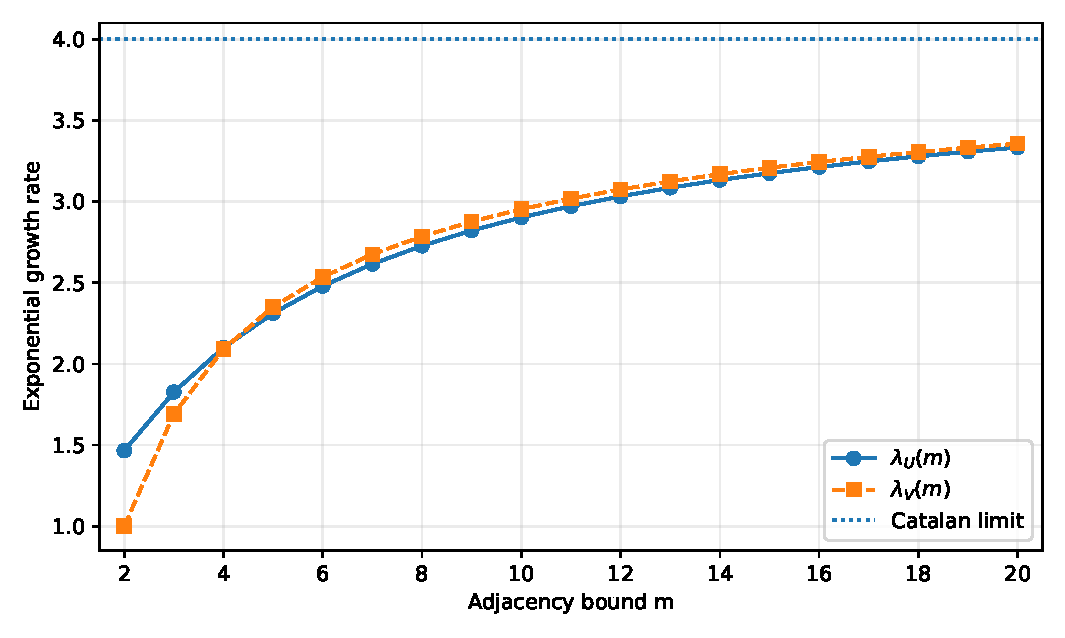
\includegraphics[width=.92\linewidth]{figures/component_growth.pdf}
\caption{The two component rates for $2\le m\le20$. Both increase, and the
component attaining the maximum changes between $m=4$ and $m=5$.
The proof of strict growth does not depend on this crossover pattern.}
\label{fig:growth}
\end{figure}

\subsection{\texorpdfstring{Large-$m$}{Large-m} scalar comparisons}
The scalar bounds can be evaluated without matrices of order $m^2$.
The implementation stores normalized Catalan coefficients
$C_k4^{-k}$, avoiding enormous intermediate Catalan integers in this
\emph{numerical} calculation. It solves for $t=m\log(4x)$, not for a root
whose distance from $1/4$ is tiny.

\begin{table}[htbp]
\centering\small
\caption{Approximate evaluation of the rigorous scalar root bounds.
The lower column is $\max_{d\in\{1,2,4,8\}}s_{m,d}^{-1}$; the upper is
$q_m^{-1}$. These decimal evaluations are floating-point results, not
outward-rounded interval certificates.}
\label{tab:scalar}
\begin{tabular}{rrr}
\toprule
$m$&Lower-bound value&Upper-bound value\\
\midrule
10&2.7001330054&3.2847596398\\
20&3.2358742549&3.5390478302\\
50&3.6448786614&3.7589497022\\
100&3.8065234928&3.8581087164\\
1000&3.9751398963&3.9790979985\\
10000&3.9969422752&3.9972999790\\
100000&3.9996392834&3.9996731933\\
1000000&3.9999586173&3.9999618975\\
\bottomrule
\end{tabular}
\end{table}
\begin{figure}[htbp]
\centering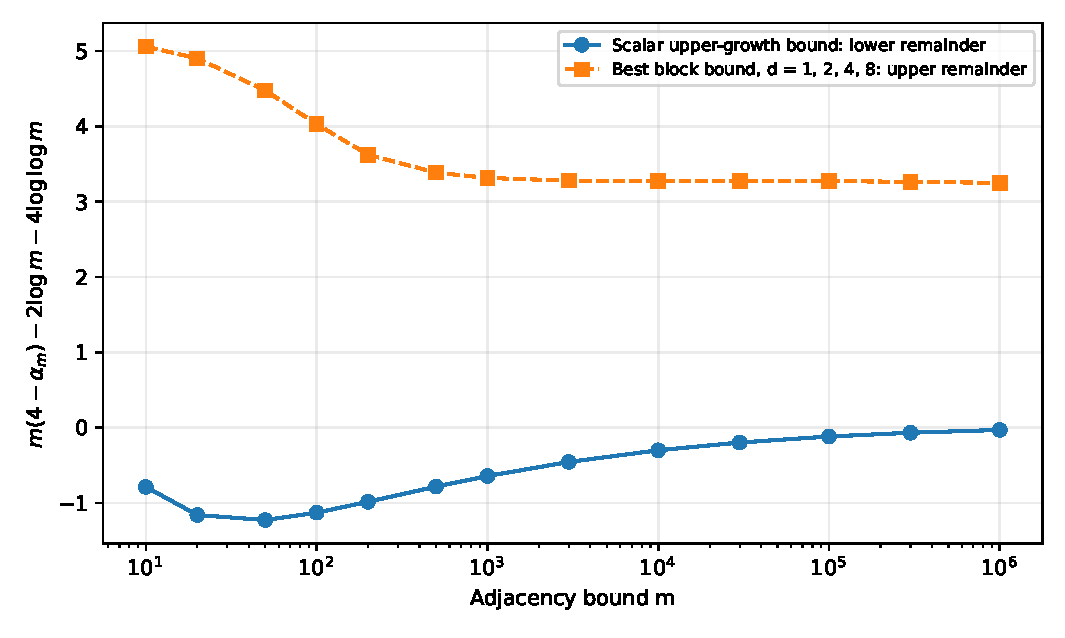
\includegraphics[width=.94\linewidth]{figures/scalar_remainder_bounds.pdf}
\caption{Numerical evaluations of the scalar bounds on the centered
remainder $E_m$. The plotted upper envelope uses only $d=1,2,4,8$.
Neither curve is the true remainder, and the asymptotic constants in
\eqref{eq:constant-window} are not finite-$m$ interval bounds.}
\label{fig:remainder}
\end{figure}

\subsection{What was actually checked}
The bundled \texttt{verification\_log.txt} records a successful complete
run of the standard-library verifier. Its checks include direct
triple-definition testing of all permutations through length seven against
the Catalan generator; the first-entry formula for every Catalan avoider
through length ten; 2,840 cumulative endpoint counts for $m=1,\ldots,8$;
and 53,534 weighted-edge comparisons under the shift for
$m=2,\ldots,30$. Both component graphs are also tested for strong connectivity
in those finite cases.

The verifier checks coefficientwise scalar majorants and block lower bounds
through $n=100$ for $m=2,\ldots,12$ and the admissible tested values of $d$.
It validates the 38 rational Perron intervals using 3,458 strict integer
row inequalities, then compares their endpoints as exact fractions.
Finally, it checks all four full polynomial-matrix certificates and compares
the resulting generating-function coefficients with the recurrence through
$n=200$.

For certificate checking, the verifier reconstructs states and weighted
edges separately, using Catalan convolutions in place of the binomial
formula used by the numerical matrix builder. It also checks agreement
between these two implementations. This reduces the risk that a common
implementation error merely reproduces itself. Nevertheless,
finite computational checks are supplements to, not replacements for,
the universal arguments in \cref{sec:strict,sec:root-lemma,sec:asympt}.

\section{What is resolved, and what remains}
\label{sec:remaining}
The strict inequality $\alpha_{m+1}>\alpha_m$ is proved for every positive
integer $m$. Together with the existing fixed-bound results, it completes
the growth-constant conjecture selected here. The scalar comparison proof
also determines the leading constant and next logarithmic term in the
approach to four.

Several nearby questions are not resolved by these arguments. The first
is whether $\lambda_V(m)>\lambda_U(m)$ for \emph{every} $m\ge5$; the reverse
inequality holds for $m=2,3,4$. This is the separate component-comparison
problem formulated in \cite[Problem~P3]{MayamaAkita}. Strict increase in
both sequences is compatible with crossings, so it cannot settle their
ordering. The finite certificates here establish the pattern only through
$m=20$.

A second question is whether $E_m$ converges, and, if so, to which constant.
The scalar majorant discards endpoint compatibility, while the lower
construction permits only a special recoverable family of blocks. Their
limiting constants leave a window of width $4\log2$. Closing that gap
requires controlling more of the endpoint information, not merely taking
more terms of the same scalar expansions. A growing-$d$ analysis could
improve finite bounds, but our argument deliberately takes $d$ fixed and
then sends $d$ to infinity only after a limsup.

Finally, the minimal recurrence order and uniform denominator factorization
of $A_m(x)$ remain outside the scope of this report. The exact $m\le4$
artifacts are useful examples, not a claimed solution of that general
algebraic problem. The new strict-growth argument is valuable precisely
because it avoids needing such a formula.

\appendix
\section{Exact small-bound algebra}
\label{app:algebra}
For $m=3$, the certified generating function is $A_3(x)=P_3(x)/Q_3(x)$, where
\begin{align*}
 P_3(x)={}&1-x-x^2+x^3+4x^4-4x^6-3x^7-3x^8\\
          &-5x^9-3x^{10}+2x^{11}+2x^{12},\\
 Q_3(x)={}&(x-1)(x+1)
 (x^5-x^4-x^3+x^2-2x+1)\\
          &\hspace{12mm}\cdot(x^6+x^5+x^4+2x^3+x^2-1).
\end{align*}
For $m=4$, the denominator factors as
\begin{align*}
 Q_4(x)={}&(x-1)\,D_U(x)\,D_V(x),\\
 D_U(x)={}&x^{10}+x^8+x^7-6x^5-x^4-x^3-x^2-x+1,\\
 D_V(x)={}&x^{12}-x^{11}-x^{10}-x^9+5x^8+4x^7+4x^6\\
          &+4x^5+5x^4+3x^3+x^2-1.
\end{align*}
Both displayed full denominators have constant term one. The numerator
of $A_4$, listed from constant term upwards, has coefficient vector
\[
\begin{gathered}
(1,-1,-1,-1,2,9,5,-3,-14,-10,-13,-23,\\
 -31,-11,21,32,21,1,-3,-5,-3,-3).
\end{gathered}
\]
It has degree 21 and $Q_4$ has degree 23. Thus the usual coefficient
recurrence from $Q_4A_4=P_4$ is valid for all $n\ge23$ when written using
23 preceding terms. The complete ascending coefficient arrays, full state
certificates, and exact checks are in the JSON files.

\section{Reproduction and certificate formats}
\label{app:reproduction}
The archive is arranged as follows:
\begin{lstlisting}
article.tex, article.pdf       Main editable source and report
README.md, requirements.txt   Reproduction instructions
code/model.py                 Exact endpoint model and combinatorics
code/compute.py               Numerical proposals and exact symbolic solver
code/verify.py                Standard-library independent exact verifier
code/plot_results.py          Recreates the two separate figures
data/sequences.csv            n = 0..200, m = 1..12
data/growth_constants.csv     Components for m = 2..20
data/perron_certificates.json Rational bounds and positive integer vectors
data/symbolic_certificate_m*.json  Polynomial state certificates, m = 1..4
data/generating_functions.json     Reduced rational functions, m = 1..4
data/large_m_scalar_bounds.csv     Scalar evaluations through m = 1000000
\end{lstlisting}

The primary reproducibility command needs no third-party Python packages:
\begin{lstlisting}
python code/verify.py
\end{lstlisting}
To regenerate numerical and symbolic proposals, install the packages in
\texttt{requirements.txt} and run
\begin{lstlisting}
python code/compute.py --max-m 20 --symbolic-max 4 --large-scalars
python code/verify.py
python code/plot_results.py
\end{lstlisting}
The generator deliberately raises an exception if it cannot convert a
numerical proposal to a valid exact certificate. A floating-point result
alone is never accepted as a proof of a spectral inequality.

To build the report from the supplied figures:
\begin{lstlisting}
pdflatex -interaction=nonstopmode -halt-on-error article.tex
pdflatex -interaction=nonstopmode -halt-on-error article.tex
pdflatex -interaction=nonstopmode -halt-on-error article.tex
\end{lstlisting}
The third pass settles page references and the table of contents if needed.
The TeX source uses standard packages from a current full TeX Live
installation; no font files are distributed.

The exact recurrence uses $(m+1)^2$ endpoint states and at most $m+1$
terms per state. Computing all coefficients through length $N$ therefore
uses $O(Nm^3)$ integer multiply-add operations, after coefficient
precomputation, and $O(Nm^2)$ stored integers in the supplied straightforward
implementation. These are arithmetic-operation counts, not bit-complexity
bounds. Exact values have growing bit length. A rolling buffer can reduce
storage when the complete coefficient table is not needed.

Perron certificates store integers $p,D$ for each radius endpoint $p/D$,
and a positive integer vector in the state order generated by the verifier.
Symbolic certificates store all polynomial coefficients in ascending degree.
The constant term of each common denominator is checked to be one.
The certificate identities prove infinitely many coefficients because the
formal system has a unique solution; the finite coefficient checks are
additional consistency tests.

\section{Source status and proof audit}
\label{app:status}
The literature check was performed on September 19, 2026. The inspected
primary items are the arXiv v1 versions listed below, including Nadler's
Conjecture~2 and Mayama--Akita's Theorem~4.14 and Problem~P3. The latter
paper's displayed numerical table and statement that its component comparison
was unproved were also inspected in the PDF. Targeted searches used the
paper titles and identifiers together with strict monotonicity, growth
constants, and asymptotic refinements. No later solution was located in
that search. This establishes the specific source-based status used here;
it is not an assertion that every possible publication has been searched.

The logical dependencies of the new claims are particularly short.
The strict-growth theorem uses the exact endpoint recurrence, the two
irreducible components, their root characterization, the proper-principal
Perron lemma, and the explicit shift of thresholds. This report includes
proofs of those prerequisites. The asymptotic theorem instead uses the
maximum-decomposition majorant, the injective skew-block construction,
the first-entry Catalan formula, and the truncated-tail lemma. In particular,
no numerical fit, unproved component-ordering pattern, or formal passage
from finite checks to all $m$ is used.

The work has not been formalized in a proof assistant. The integer and
polynomial certificates are executable verification of the stated finite
algebraic claims; they should not be described as a formal verification
of the analytic limiting argument or of the all-$m$ theorem.

\begin{thebibliography}{9}
\bibitem{Nadler}
N. Nadler, \emph{On 132-Avoiding Permutations with an Adjacency Constraint},
arXiv:2604.22135v1, submitted April 24, 2026.
\url{https://arxiv.org/abs/2604.22135}.
Conjecture~2 is in Section~5.2.

\bibitem{MayamaAkita}
T. Mayama and D. Akita, \emph{Finite-state enumeration of adjacency-constrained
132-avoiding permutations}, arXiv:2605.23519v1, submitted May 22, 2026.
\url{https://arxiv.org/abs/2605.23519}.
Relevant locations: Theorem~2.4, Proposition~2.7, Theorems~4.12 and~4.14,
and Problem~P3 in Section~5.
\end{thebibliography}
\end{document}
